% Copyright (c) 2008-2009 solvethis
% Copyright (c) 2010-2016,2018-2019,2021 Casper Ti. Vector
% Copyright (c) 2021 Kurapica
% Copyright (c) 2021 iofu728
% Overleaf version.
%
% 当前overleaf 版本字体和格式均符合2021硕士学位论文要求
%
% 该版本遵循北京大学研究生学位论文写作指南2019年v2版本、北京大学硕士研究生学位论文word模板,
% 在CasperVector/pkuthss模板的基础上针对硕士研究生学位论文格式的要求进行相应修改,
% 遵循 LaTeX Project Public License 和 知识共享 署名 - 非商业性 - 相同方式共享 4.0 国际协议
% 如有任何疑问请在github/iofu728/pkuthss上提问或联系作者iofu728。
%
% 此处请保留 ugly 参数,参考文献管理采用GB/T 7714-2015标准。
% 此处使用顺序编码制,如使用著者-出版年制则更改为b7714-2015av。
% bib引用使用基本与日常学术论文写作相同,部分略有不同,
% 参考https://github.com/hushidong/biblatex-gb7714-2015/blob/master/example/cls-beamer.tex
\documentclass[UTF8,nocolorlinks,ugly]{pkuthss}
\usepackage[backend=bibtex,bibstyle=gb7714-2015,citestyle=gb7714-2015]{biblatex}
\setlength{\bibitemsep}{3bp}
\renewcommand*{\bibfont}{\zihao{5}\linespread{1.27}\selectfont}

\pkuthssinfo{
	cthesisname = {人类生存发展与核科学课程作文},
 	thesiscover = {人类生存发展与核科学作文},
	ctitle = {简述核聚变的原理及应用},
	cauthor = {吴熙楠},
	studentid = {1900011413},
	date = {\zhdigits{2021}\ \ 年\ \ \zhnumber{5}\ \ 月},
	school = {物理学院},
	% 副教授 A.P. 讲师 Lect.
	cmentor = {郭秋菊\ \ 教授},
	ckeywords = {核聚变,新能源,核能文明}
}
\addbibresource{ref.bib}


\begin{document}
	\frontmatter
	\pagestyle{empty}
\maketitle
\cleardoublepage
\pagestyle{plain}
\setcounter{page}{0}
\pagenumbering{Roman}
\begin{cabstract}
	在人类社会现代化进程中,文明的发展与能源的开发紧密相连,尤其是近一百年来,人们对能源的开发远胜于前,现有的化石燃料及新能源难以长久满足人类的需要,这时候核聚变能这个具有巨大潜力的新能源便成了目前发展新方向。虽然目前核聚变能的利用技术不够成熟,还有很多困难有待克服,但核聚变能作为新能源的崛起必然是时代潮流,人类必将从“石油文明”走向“核能文明”。
\end{cabstract}

% vim:ts=4:sw=4

\tableofcontents

	\mainmatter
	\chapter{背景}
1492年,当哥伦布发现新大陆时,世界人口为4.5亿(相当于今天人口的6.5\%),世界能源消耗还不到今天的1\%。世界人口稀少,能源充足可以支持文明发展。18世纪中叶,蒸汽机的发明开启了工业革命,20世纪初,爱因斯坦的质能方程使人类能够控制原子内部的各种过程,从而发展出各种现代新技术,因此,能源消耗也随之增加,人口也随之增加。目前,世界人口从哥伦布时代的4.5亿增长到70亿,在过去的100年里,世界人口增长了4倍,而能源消耗增长了10倍,即,能源消耗的增长快于人口增长,但是为了满足人们不断增长的物质文化需要,这种人均能源消费增长的趋势必然会继续下去。\cite{Lee2011NuclearFE}
\par 在过去的100年中,世界人口翻倍的时间约为50年,但能源消耗翻倍的时间约为30年。如果这个趋势继续下去,世界将会达到能源供应的临界点。因为能源资源是有限的,据估计供应趋势将在今后短短几十年内达到顶峰。我们需要开发一种新的无限的能源,并且清洁无污染的能源,不会污染环境。这时候我们想起了爱因斯坦的质能方程,核裂变和核聚变将会是一种不错的选择。但是对于核裂变反应,我们将会一直有放射性核废料积累,这显然不是长久之计。而对于核聚变,这与在恒星中发生的过程相同,将会利用质量亏损而产生的巨大的能量,并且因为使用的不是放射性元素,因此不会有核裂变的放射性安全隐患;而用于核聚变的燃料,锂和氘不仅无污染,而且因为海水中有丰富的锂,各种形式的水中也有丰富的氘,原料也十分容易获取。因此,核聚变能量的应用前景是非常优秀的。

	\chapter{核聚变原理}
20世纪初爱因斯坦发现质能方程,人们由此发现了原子核核能的巨大潜力。根据质能方程$E=mc^{2}$,原子核净质量变化将会造成能量的释放。如果有多个重的原子核变化为多个轻的原子核,称为核裂变,如原子弹爆炸;如果是由较轻的原子核变化为较重的原子核,称为核聚变,因为核聚变是给大部分活跃恒星提供能量的过程,因此又称热核反应。如:两个氘发生聚变反应生成一个氢和一个氚,将会放出$4.03MeV$能量,反应方程式为:$_{1}^{2}H+_{1}^{2}H\rightarrow_{1}^{3}H+_{1}^{1}H+4.03MeV$。


核聚变将较轻的原子核结合形成较重的原子核,但是由于原子核带正电,因此原子核之间会有库仑排斥力,这将会阻碍原子核的结合,克服库仑势垒需要巨大的能量。但是由于轻核所带的电荷少,因此轻核之间发生核聚变时需要克服的势垒越小,释放出的能量就越多。



因此如果要进行核聚变反应,首先就必须提高物质的温度,让原子核与电子之间形成等离子体,但由于原子核带正电,彼此间会互相排斥,所以很难使其彼此互相接近,因此我们还必须让等离子体的温度达到超高温($\sim10^{8}K$),还需要达到一定的密度和封闭时间。由于提高物质的温度可以使原子核剧烈运动,因此温度升高,密度变大,封闭的时间越长,彼此接近的机会越大。但由于等离子体很快分散,所以必须先将其封闭。太阳内部是利用巨大万有引力使等离子体封闭,引力场约束形成简并电子气,这在地球上显然是行不通的,当然由于等离子体带电,因此我们可以合理利用磁约束来达到封闭效果。
    \chapter{核聚变能的前景}
\section{核聚变能的优势}
\subsection{核聚变释放的能量巨大}
众所周知,在化学反应中,我们在获取能量的过程中,例如石油、天然气燃烧,每涉及到一对原子,只能得到$eV$量级的能量(一个可见光光子能量量级)。这取决于外部原子电子的结合能在$eV$范围内。但是在另一方面,在核转换过程中,我们通过爱因斯坦的质能关系,每一对核所能吸收或释放的能量量为$MeV$。因此,对于每获得一定量的能量,核反应转化的质量大约是燃烧所需质量的百万分之一。因此,对于原子核来说,每一个稳定的原子核的质量都比其所有组成部分(质子和中子)的质量之和要低\cite{Focardi2010ANE}。而相对于核裂变而言核聚变也能产生更多的能量,如果燃料的质量相等,核聚变释放的能量是裂变的3到4倍\cite{Petrescu2017SomePS}。因此在释放能量的“性价比”方面,核聚变显然是目前最具潜力的新能源。
\subsection{核聚变原料充足}
核聚变的原料相对于普通化石燃料而言充足得多,现代普遍估计在全球的化石燃料将在$100\sim 200$年内达到临界值,到时候将会把所有化石燃料消耗光。但是对于核聚变而言,如氘和氚之核聚变反应,其原料可直接取自海水(海洋自然包含这样一个大规模的氘($33g/m^{3}$)),氘在海洋中相当丰富,海洋中每$1km^{3}$海水中氘原子所具有的潜在能量相当于燃烧13600亿桶原油的能量,这个数字约为地球上蕴藏的石油总储量,而且海洋中的锂也可以用来提供核聚变的燃料,理论上用氘和氚进行核聚变可以满足当前的能源消耗人类一亿年的使用,这样几乎可以说是原料无穷无尽了,因此对于核聚变能而言我们几乎不用考虑能源原料问题。
\subsection{核聚变能为清洁安全的能源}
首先,相较于普通化石燃料,核聚变不会产生温室气体,因此也不会造成温室气体带来的全球环境问题;第二,相较于核裂变发电,核聚变产生的核废料半衰期极短(低管理成本、核泄漏时总危害较低)、安全性也更高(不维持对核的约束便会停止反应),而且与核裂变不同(核裂变用作燃料的原材料具有放射性,核裂变产生的能量也对应着放射性废料的产生),核聚变产物本身(主要是$_{2}^{4}He$)没有放射性,但当反应用来释放快中子时,它们可以将捕获它们的原子核转化为同位素,其中一些是放射性的。同时核聚变也是一种中子源,借此可以触发核裂变,这被称为次临界核裂变,次临界核裂变不但安全性接近核聚变,且技术难度较核聚变发电低,还可以处理核裂变发电造成的核废料问题,让这些核废料的半衰期由数万年缩短为数百年,可以说是一举多得。
\section{核聚变能的劣势}
\subsection{核聚变的严苛条件}
虽然看起来从理论上来讲核聚变反应能为人类提供无穷无尽的能量来源,但实际上我们现在还没能做到可以商业化生产的可控核聚变堆,这是因为核聚变反应所需要的严苛的反应条件与技术要求。


首先,在原理部分我们也提到了,需要克服库仑势垒,我们需要外界给一个强力的能量来源,比如我们需要提供$10^{8}K$的超高温(冷核反应由于实验室无法重现故不与讨论),而我们目前的加热效率低下,我们目前主要是等离子体电流加热,但是由于电子与等离子体碰撞的能量损耗太大,且普通导体的允许临界电流密度太小,因此我们用这种方法加热的效率低下,且难以实现。而惯性约束核聚变与磁约束核聚变目前还不是特别稳定,技术不够成熟,距离真正实用还有一段路要走。
\subsection{核聚变的“放射性”}
虽然核聚变能比核裂变能清洁,但是为了易实现核聚变, 需要使用放射性氖,既然用了放射性原料,会发生放射性污染的危险。而且核聚变反应产生的中子可以跟反应装置的墙壁发生核反应,因为这种聚变堆部件承受着极大的负荷,墙壁被中子轰击后会带有“放射性”,用一段时间之后就必须更换,而且换下来的墙壁成了核废料,这就出现如同核裂变堆那样的核废物处置问题。
    \chapter{可控核聚变的现况}
\section{国际热核聚变实验堆}
国际热核聚变实验反应堆是国际核聚变研究和巨型工程,这是目前正在建设世界上最大的实验性托卡马克核聚变反应堆,$ITER$将使用环形加速器产生温度超过$10$亿度的氢等离子体,它将产生大约$500MW$的核聚变能量,维持大约500秒;相比较而言欧洲联合环形加速器的最高纪录不过是$16MW$维持了不到1秒。作为聚变能实验堆,$ITER$要把上亿度、由氘氚组成的高温等离子体约束在体积$837m^{3}$的"磁笼"中,产生5亿瓦的聚变功率,持续时间达$500$秒。这是人类第一次获得接近电站规模的受控聚变能。


在$ITER$上开展的研究工作将揭示这种带有氘氚核聚变反应的高温等离子体的特性,探索它的约束、加热和能量损失机制,等离子体边界的行为以及最佳的控制条件,从而能够为今后建设商用的核聚变反应堆奠定坚实的科学基础。对$ITER$装置工程整体及各部件在5亿瓦聚变功率长时间持续过程中产生的变化及可能出现问题的研究,不仅将验证受控热核聚变能的工程可行性,而且还将对今后如何设计和建造聚变反应堆提供必不可少的信息。


同时值得说明的是,我国于2006年正式加入$ITER$计划,这显示了我国作为一个大国所应该有的国际担当,也显示了我国在科技领域也在逐步推行着改革开放的步伐,带动了我国不仅是核聚变领域,同时也有材料技术,激光技术以及超导技术等方面技术的提高,培养了一堆可靠的科研人才,推动了我国在科研领域的进展。
\section{中国“人造太阳”}
$EAST$是我国新时代“人造太阳”实验装置,位于中国合肥。2009年,$EAST$首轮物理放电实验取得成功,标志着我国站在了世界核聚变研究的前端。2012年4月19日,$EAST$中性束注入系统完成了氢离子束功率3兆瓦、脉冲宽度500毫秒的高能量离子束引出实验,这标志着我国自行研制的具有国际先进水平的中性束注入系统基本克服所有重大技术难关。2016年2月,$EAST$物理实验获重大突破,实现在国际上电子温度达到5000万度持续时间最长的等离子体放电。2018年,$EAST$实现1亿摄氏度等离子体运行等多项重大突破\cite{chinaEAST2}。


$EAST$相继完成了辅助加热、钨偏滤器、等离子体物理诊断等系统的升级改造,基本解决了射频波耦合、高约束等离子体稳定性控制、等离子体与壁相互作用物理、低动量条件下加热和电流驱动下输运、杂质输运和控制等问题,为实现长脉冲稳态高约束模等离子体奠定了基础,其稳态运行模式将为$ITER$和未来反应堆提供重要参考\cite{chinaEAST1}。


总的来说,我国的核科学研究虽然相较于国外起步晚,但是在我国科学家的不懈努力下,我们已经迎难而上,几乎走在了世界的前列,相信在不久后的将来我们也能够享受到核聚变能量带来的便利条件和发展了。
\section{核聚变能发展的必要性}
正如之前在背景中所描述的那样,对能源供应和消费的估计表明,本世纪中叶将是世界能源供应无法跟上需求的临界点。由于世界人口的增长和人均能源消费的增长,需求不可避免地增长;而技术经济进步与人均能源消耗密切相关。因此,能源供应不足将限制人类文明的进步,但是当核聚变技术完善到聚变燃烧氘时,即使能源消耗像过去一样持续增长,其燃料供应也将持续数百万年。而仅仅到了下个世纪,核聚变能源就应该能够填补这一空白,人类文明也能继续进步和增长。另一方面,如果没有核聚变能源,人类的命运将不可避免地严重衰退,世界人口将减少到50亿以下,最终甚至更低。如下图所示\cite{Lee2011NuclearFE}:
\begin{figure}[htb]
	\begin{center}
		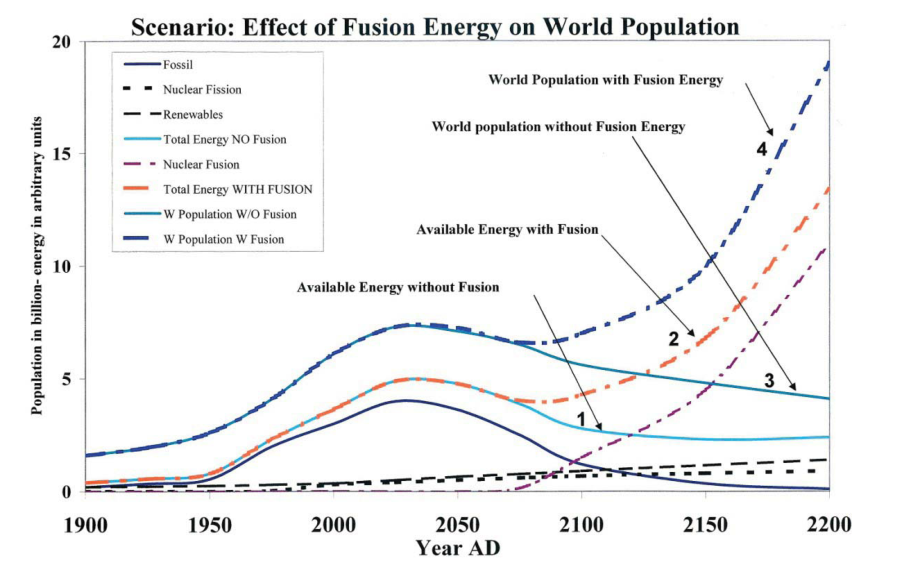
\includegraphics[width=\textwidth]{pic/n.png}
		\caption{基于人口持续增长的能源消耗图}
		\label{fig:example_img}
	\end{center}
\end{figure}
\par 从此图可以看出,核聚变能源的发展即将到来,总能源开始下降的临界点被认为是在本世纪中叶,此后,人类将不得不应对供应的减少,除非不断增加的短缺被核聚变能源弥补。到了下个世纪,核聚变能源应该能够填补这一空白,让人类文明继续进步和增长。而且由于核聚变能源的发展是一个复杂的技术任务可能会有几十年的能源短缺,这将严重影响图中的能源消费。这种能源停滞期和相应的世界人口停滞期即使在核聚变能源的发展和采用的情况下也是不可避免的。在没有核聚变能源的情况下,在此图情形下,世界人口下降到50亿以下,也就意味着人类文明的倒退。因此,为了人类以后文明的发展,核聚变能源的开发和使用是必要的。
    \chapter{总结与展望}
在本篇文章中我们从目前人口增长的大背景出发说明了核聚变这种具有巨大潜力的能源的必要性,可以说是如果我们除非移居到地外行星(然而这种方法实施的难度远大于开发核聚变能的难度),否则地球目前的可利用资源将会很快不能支持人类的需求,因此核聚变能的必要性就凸显了出来,从长远来看,核能也将是继石油、煤和天然气之后的主要能源,人类将从“石油文明”走向“核能文明”。它的优势毫无疑问是巨大的,甚至可以让人类在以后几千万年都不用为了能源问题困扰,但是它也有一些劣势,其中最为重要的一条就是核聚变的发生需要极为严苛的条件,虽然在实验室条件下我们已经可以实现可控核聚变反应堆,但是我们离真正的实用商业化还是有很长一段路要走的;同时,近年来我国在核聚变能源方面的研究与发展迅速,各国之间对于核聚变能源的研究也趋向于合作共赢,因此,可以想象在不久后的将来,我们将会见证核聚变能作为新能源的崛起,人类发展也将进入新的时代。
    \appendix  
    \printbibliography[heading = bibintoc]

\end{document}

% vim:ts=4:sw=4
